\documentclass{tikzcd}

\begin{document}
  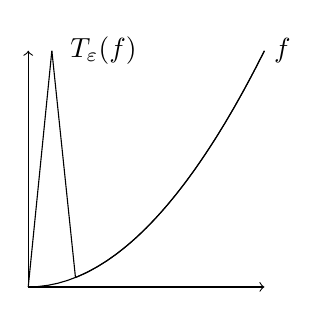
\begin{tikzpicture}[scale=3]
    \draw[->] (0, 0) -- (1, 0);
    \draw[->] (0, 0) -- (0, 1);

    \draw[domain=0:1, variable=\x] plot ({\x}, {\x^2}) node[right] {\( f \)};

    \draw (1/2, 1) node[left] {\( T_\varepsilon(f) \)};
    \draw[domain=0:0.1, variable=\x] plot ({\x}, {10 * \x});
    \draw[domain=0.1:0.2, variable=\x] plot ({\x}, {0.04 + (1 - 0.04) * (2 - 10 * \x)});
    \draw[domain=0.2:1, variable=\x] plot ({\x}, {\x^2});
  \end{tikzpicture}

  \begin{tikzpicture}[scale=5]
    \draw[->] (0, 0) -- (1, 0);
    \draw[->] (0, 0) -- (0, 1);
    \draw[domain=0:4/10, thick, variable=\x] plot ({\x}, {0});
    \draw[domain=4/10:6/10, thick, variable=\x] plot ({\x}, {5 * \x - 2}) node[left] {\( g \)};
    \draw[domain=6/10:1, thick, variable=\x] plot ({\x}, {1});

    \draw[densely dotted] (0, 6/10) node[left] {\( f_k\parens*{\frac 1 2} - \varepsilon \)} -- (1, 6/10);
    \draw[densely dotted] (0, 8/10) node[left] {\( f_k\parens*{\frac 1 2} + \varepsilon \)} -- (1, 8/10);

    \draw[densely dotted] (4/10, 0) -- (4/10, 1);
    \draw (3/10, -1/10) node {\( \frac {1 - \delta} 2 \)};
    \draw[densely dotted] (1/2, 0) -- (1/2, 1);
    \draw (1/2, -1/10) node {\( \frac 1 2 \)};
    \draw[densely dotted] (6/10, 0) -- (6/10, 1);
    \draw (7/10, -1/10) node {\( \frac {1 + \delta} 2 \)};

    \draw[domain=-1/10:1, dash dot, variable=\x] plot ({\x}, {2/10 + 1 / (1 + e^(5/3*(1-2*\x)))}) node[right] {\( f_k \)};
  \end{tikzpicture}
\end{document}
